\chapter{Mod�le du syst�me}



\section{Cas d'utilisation}




\section{Diagramme de classes}

Notre  projet  s'architecture autour  d'une  classe principale  nomm�e
Agent.  Le diagramme  UML  de  classes est  disponible  sur la  figure
\ref{fig:diagramme_classes}.

\begin{figure}[ht]
  \centering
  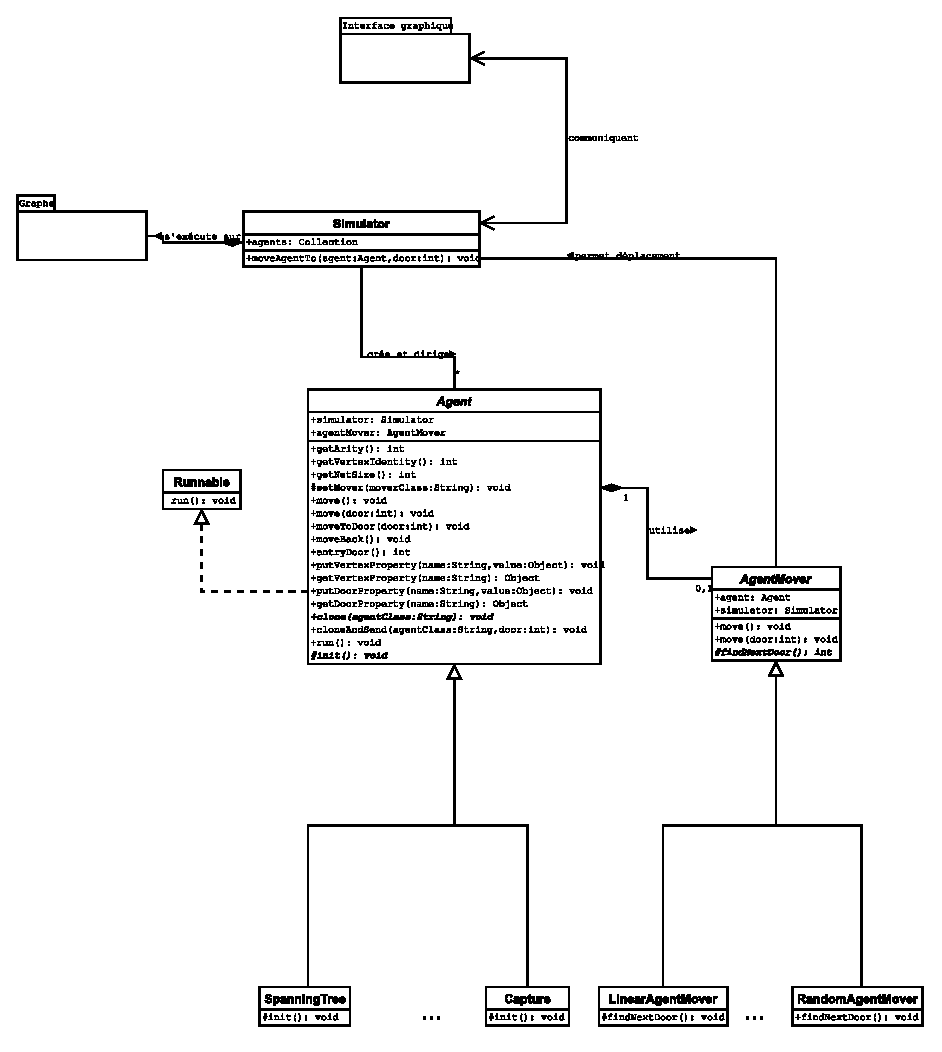
\includegraphics[width=14cm]{figures/classes}  
  \caption{Diagramme de classes}
  \label{fig:diagramme_classes}
\end{figure}


\subsection{La classe Agent et ses sous-classes}

La  classe  Agent  impl�mente  toutes les  m�thodes  n�cessaires  pour
faciliter  le  travail du  futur  d�veloppeur  d'agents mobiles.   Les
m�thodes  seront d�critent  dans  la partie  \ref{sec:api}  � la  page
\pageref{sec:api}.\\

De fa�on g�n�rale, on peut  trouver des m�thodes d'informations sur le
graphe, des m�thodes  de gestion de propri�t�s (au  niveau des sommets
et des portes), des m�thodes de d�placements et de clonage.\\

Le futur d�veloppeur devra,  pour impl�menter ses agents, sous-classer
cette classe Agent et impl�menter les deux m�thodes abstraites : \\

\begin{description}
\item[init]   Utilis�e pour impl�menter le code g�n�ral de
  l'algorithme. C'est  cette m�thode  qui sera lanc�e  lorsque l'agent
  sera ex�cut�.
\item[clone]  Sert  �  retourner   un  nouvel  Agent  ayant  les  m�me
  caract�ristiques. 
\end{description}

%% Local Variables:
%% mode: latex
%% coding: latin-1
%% TeX-master: "main"
%% End:
